\documentclass[border=8pt]{standalone}
\usepackage{amsmath}
\usepackage{fontspec}
\setmainfont{Source Serif 4}
\usepackage{tikz}
\usetikzlibrary{positioning, arrows.meta}
\definecolor{qbase}{RGB}{31,86,160}
\definecolor{winner}{RGB}{209,73,91}

\begin{document}
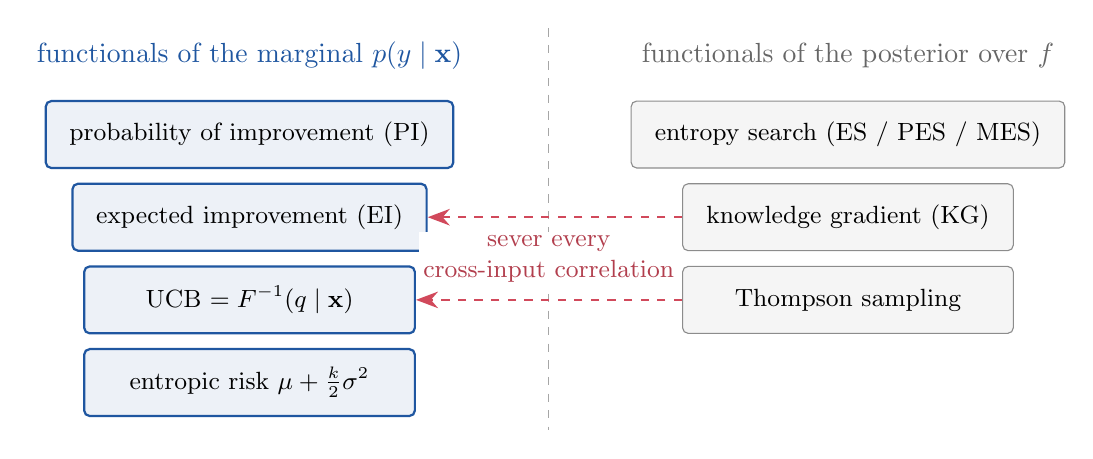
\begin{tikzpicture}[
  font=\small,
  box/.style={draw, rounded corners=2pt, minimum height=8.5mm, minimum width=42mm,
              inner xsep=3mm, inner ysep=2mm, align=center},
  bbox/.style={box, draw=qbase, fill=qbase!8, thick},
  gbox/.style={box, draw=black!45, fill=black!4},
  collapse/.style={-{Stealth[length=2.8mm]}, winner, thick, dashed},
]
% headers
\node[font=\normalsize, qbase, align=center] at (2.6, 1.0)
  {functionals of the marginal $p(y \mid \mathbf{x})$};
\node[font=\normalsize, black!60, align=center] at (10.2, 1.0)
  {functionals of the posterior over $f$};
% the divide
\draw[dashed, black!35] (6.4, 1.35) -- (6.4, -3.75);
% marginal side
\node[bbox] (pi) at (2.6, 0) {probability of improvement (PI)};
\node[bbox] (ei) at (2.6, -1.05) {expected improvement (EI)};
\node[bbox] (ucb) at (2.6, -2.1) {UCB $= F^{-1}(q \mid \mathbf{x})$};
\node[bbox] (ent) at (2.6, -3.15) {entropic risk $\mu + \tfrac{k}{2}\sigma^{2}$};
% posterior side
\node[gbox] (es) at (10.2, 0) {entropy search (ES / PES / MES)};
\node[gbox] (kg) at (10.2, -1.05) {knowledge gradient (KG)};
\node[gbox] (ts) at (10.2, -2.1) {Thompson sampling};
% residues under severed correlations
\draw[collapse] (kg.west) -- (ei.east);
\draw[collapse] (ts.west) -- (ucb.east);
\node[winner!85!black, font=\small, align=center, fill=white, inner sep=1.5pt] at (6.4, -1.58)
  {sever every\\ cross-input correlation};
\end{tikzpicture}
\end{document}
